\documentclass[../main/report.tex]{subfiles}
\begin{document}
\begin{figure}[H]
	\centering
	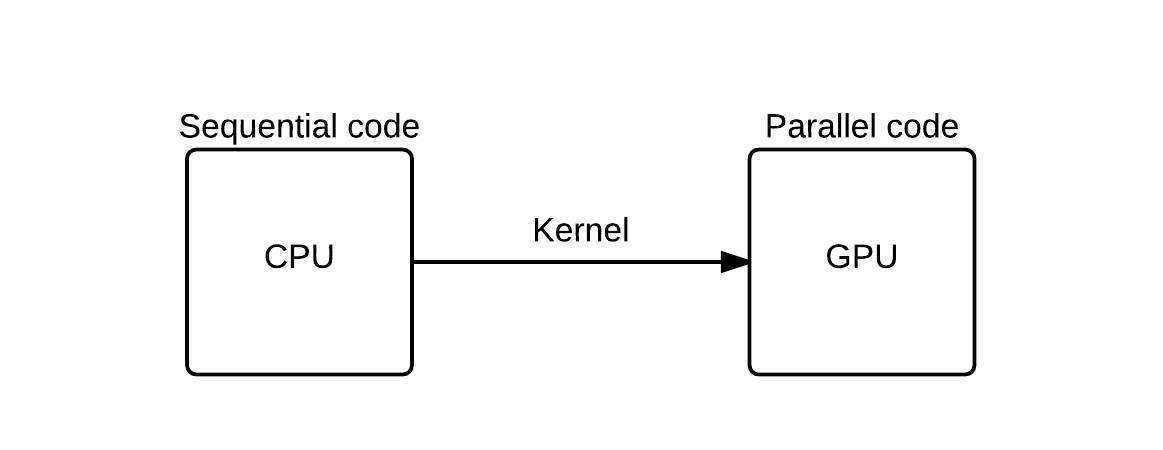
\includegraphics[width=\textwidth]{../system_overview/diagrams/programming_model_cpu_gpu.png}
	\caption{Relationship between CPU and GPU code.}
	\label{fig:programming_model_cpu_gpu}
\end{figure}

\todo{That sentence is a bit dangling and not part of the rest of the chapter. Maybe talk more about CUDA/OpenCL before we start explaining?}
The programming model for Demolicious has been heavily inspired by CUDA and OpenCL, 
and readers with programming experience with those technologies will find much of this chapter familiar.

Many applications can be divided into sequential and parallel parts,
where the characteristics of each part make them benefit from different hardware.
On the Demolicious system, the sequential parts of a program will be run by the CPU, and the parallel parts can be performed by the GPU through kernels.
\todo{Mention SIMT}
A kernel is a simple program meant to be executed by multiple threads.
The kernels are uploaded to the GPU, and then executed when requested by the CPU.
This interaction allows for programs that consist of both parallel and sequential tasks, such as graphics applications.
\todo{Replace last sentence}

\subsection{Kernels}
The GPU can start a massive amount of threads executing the same kernel.
Each thread executing the kernel is assigned a unique thread id.
The thread id can be used to compute memory addresses and make control decisions.
This allows threads to behave differently even though they are executing the same code.

To best illustrate the programming model, a few examples will be walked through.
Let's start with a simple one; fill the screen with the color green.
We assume that the pixel color values are stored in memory from location 0 and upwards.
In a sequential programming model one would typically write a loop that would fill
the memory locations with the value for green one by one.
This can be seen in listing \ref{sequential-green}.

\begin{c-code}[caption=A sequential program filling the screen with green, label=sequential-green]
int green = 0x00FF00;
for (int i = 0; i < nr_of_pixels; i++){
    write(i, green);
}
\end{c-code}

However, in the SIMT programming paradigm which our architecture is inspired by,
you write a \emph{kernel} that fills only a single pixel with green, 
and then run it with one thread for every pixel.
Below, in listing \ref{lst:green-kernel}, 
a kernel written for Demolicious that fills a single memory location,
or pixel, with green is presented.
The memory location to be written to is decided by the special id register.


\begin{assembly}[caption=A simple kernel that fills the screen with the color green, label=lst:green-kernel]
ldi $data, 0b0000011111100000
mv $address_lo, $id_lo
mv $address_hi, $id_hi
sw
thread_finished
\end{assembly}

Let's walk through the kernel one line at a time.
The first line uses the \verb/ldi/ instruction, which stands for load immediate.
It loads the value 0b0000011111100000,
which corresponds to the color green in the Demolicious color space,
into the special register \textbf{\$data}.
The second and third line move the kernel's thread ID into the address registers.
This means all pixels starting with address zero and up until the number of executed threads
will get colored green.
Finally, the store instruction is executed, storing the value in the \textbf{\$data} register
to the address given by the two address registers.
The thread stops running after executing the \verb/thread_finished/ instruction.

Now, how do we execute this kernel on the GPU?
The program running on the CPU, referred to as the \emph{host program},
has to upload the assembled kernel, and then notify the GPU to run it.
Kernels can be assembled using a custom-built assembler,
which translates special registers and pseudo instructions, and outputs as c arrays for convenience.

\begin{c-code}[caption=Loading and executing a kernel, label=lst:load-kernel]
instruction_t fill_screen_kernel[] = {
    0x08050000, // ldc $data, 0
    0x00402004, // mv $address_lo, $id_lo
    0x00201804, // mv $address_hi, $id_hi
    0x10000000, // sw
    0x40000000 // thread_finished
};

kernel_t fill_screen = load_kernel(fill_screen_kernel);

run_kernel(fill_screen, 4096);
\end{c-code}

In listing \ref{lst:load-kernel}, we first see the assembled kernel stored in the
\verb/fill_screen_kernel/ array.
It is then uploaded to the GPU using the \verb/load_kernel/ function.
A reference to the uploaded kernel is returned, which can be used when running the kernel.
In addition, the \verb/run_kernel/ function needs to know the number of threads to spawn.
Here, we spawn 4096 threads, enough to color 64*64 pixels green.

While being able to make the screen green by running a specialized kernel is nice,
it would require many very similar kernels to color the screen in different colors.
To improve on this, kernels can take parameters as input,
which lets them be reused with varying output.
The CPU can set these parameters to different values each time a kernel is run.
For instance, the CPU can set the desired color as a parameter,
and the kernel will store that value to memory instead of a predefined immediate.
Listing \ref{lst:param-color-kernel} shows an example kernel where the color is stored as a parameter.

\begin{assembly}[caption=A kernel loading the color value from a parameter, label=lst:param-color-kernel]
ldc $data, 0
mv $address_lo, $id_lo
mv $address_hi, $id_hi
sw
thread_finished
\end{assembly}

The only changed line in this kernel is the first one,
where instead of using an immediate value, we load a value using the \verb/ldc/ (load constant) instruction.
The value is a constant from the kernel's viewpoint, as it cannot be changed from the GPU.
Instead, the value is set from the CPU using the \verb/load_constant/ function,
as seen in listing \ref{lst:kernel-constant}.

\begin{c-code}[caption=Now drawing a blue screen using parameters, label=lst:kernel-constant]
load_constant(0, 0x001F);
run_kernel(fill_screen, 4096);
\end{c-code}

The instruction set available to kernels is fairly limited.
Most notably, the control flow in kernels is linear, meaning they cannot do any branches or jumps.
Although the kernels don't support diverging control flow,
conditional execution is accomplished through predicated instructions.

Each of the instructions in the instruction set can be executed conditionally by prefixing them with \emph{?}.
Whether a conditional instruction is executed is controlled by a dedicated masking register.
The programmer may use arithmetic and logic operations to manipulate this register (such as the \verb/srl/ instruction in listing \ref{lst:masked-execution}).
The mask register is only one bit, so only the least significant bit of data written to it will be stored.
A masked instruction is not executed if the mask register is \textbf{1}.

\begin{assembly}[caption=Conditional execution using predicated instructions, label=lst:masked-execution]
ldc $10, 0 ; Load color one
ldc $11, 1 ; Load color two
srl $mask, $id_lo, 6 ; Shift to the right converts ID to y pos
mv $data, $10 
? mv $data, $11 ; Will only be executed every other row
mv $address_lo, $id_lo
mv $address_hi, $id_hi
sw
thread_finished
\end{assembly}

The kernel starts with loading two color parameters.
It then stores a shifted thread ID into the mask register.
Shifting a thread ID to the right is a trick to convert the ID to a y value,
which works when the screen width is a power of two.
The mask register is only 1 bit, and will just store the least significant bit written to it.
This means that masking will be enabled for odd rows and disabled for even rows.
Line 4 first writes a color value to the \textbf{\$data} register.
When masking is disabled this value will be overwritten on line 5.
The kernel finishes by writing the data value to memory.

\todo{Talk about memory and cooldown}

\end{document}
